%%%%%%%%%%%%%%%%%%%%%%%%%%%%%%%%%%%%%%%%%%%%%%%%%%%%%%%%%%%%%%%%%%%%%%%%%%%%%%%%
%2345678901234567890123456789012345678901234567890123456789012345678901234567890
%        1         2         3         4         5         6         7         8

\documentclass[letterpaper, 10 pt, conference]{ieeeconf}  % Comment this line out
                                                          % if you need a4paper
%\documentclass[a4paper, 10pt, conference]{ieeeconf}      % Use this line for a4
                                                          % paper

% \IEEEoverridecommandlockouts                              % This command is only
%                                                           % needed if you want to
%                                                           % use the \thanks command
\overrideIEEEmargins
% See the \addtolength command later in the file to balance the column lengths
% on the last page of the document



% The following packages can be found on http:\\www.ctan.org
\usepackage{graphicx} % for pdf, bitmapped graphics files\
\usepackage{subcaption}
\usepackage{amsmath}
\usepackage{booktabs}
\usepackage{hyperref}

\title{\LARGE \bf
Hing-King-Linden Score: 
A robust method of assessing foosball matchups independent of tournament structure
}

\author{Philip Linden, Adam King and Brandon Hing% <-this % stops a space
}

\begin{document}

\maketitle
\thispagestyle{empty}
\pagestyle{empty}


%%%%%%%%%%%%%%%%%%%%%%%%%%%%%%%%%%%%%%%%%%%%%%%%%%%%%%%%%%%%%%%%%%%%%%%%%%%%%%%%
\begin{abstract}

The results of randomly seeded single-elimination tournaments does not reflect a player or team's relative rank, or foosball performance score. 
Existing ranking such as Elo Ranking or Swiss systems depend on a large number of matches to be played to produce accurate results. 
We present a method of determining rank using the relative performance of a player's opponent and the points scored on that opponent during a foosball match.
We demonstrate that the Hing-King-Linden Score, or HKL, is a robust method of predicting foosball matchups between two players or teams, and a reliable way to seed teams and tournaments fairly based on only the number of matches played and tracking points scored against each opponent.
We show the utility of HKL using the real results of a randomly seeded single-elimination tournament.

\end{abstract}


%%%%%%%%%%%%%%%%%%%%%%%%%%%%%%%%%%%%%%%%%%%%%%%%%%%%%%%%%%%%%%%%%%%%%%%%%%%%%%%%
\section{INTRODUCTION}

Championship tournaments are a tried-and-true organization for competitions in sports today, and foosball is no exception. 
However, both single- and double-elimination tournament results are predicated upon fair seeding of the matchups at the start of the tournament.
Some existing ranking systems used to seed tournaments are Elo Ranking\cite{}, used for the FIFA World Cup\cite{}, or the Swiss-system\cite{}, commonly used in chess tournaments\cite{}.
A fair score in both Elo and Swiss systems requires that each member of the tournament plays every other in round-robin fashion, where $\frac{n}{2}(n-1)$ matches must be played before a rank is determined. 
The difference in these rankings is in how scores incorporate margin of victory and win/loss rates.
Additionally, existing rating systems assume that results are binary (win or loss) or uncapped scores (higher score wins). In foosball, wins are determined by the first team to score a set number of points. 

In a recent tournament, the competition organizers used a single-elimination tournament between 16 randomly seeded players to seed an 8-team tournament of evenly matched 2-person teams. 
In this event structure, we must determine relative skill of 16 players when the conditions for Elo and Swiss rankings systems are not met---not only have players not played at least one match against one another, but some players played more matches than others. In some cases, players eliminated in the first round scored more points and lost by a smaller margin of victory against the overall winner of the tournament. Thus it is clear that a robust ranking system is needed to assemble fair teams based on match results using the relative performance of a player's opponent to determine that player's rank.

In this paper we propose the Hing-King-Linden Score, or HKL, which weighs the cumulative number of points scored against each opponent and the relative performance of that opponent. 
Critically, HKL only requires one randomly seeded single-elimination tournament to determine an accurate score that reflects relative performance. 

The primary goal of the HKL is to rank contestants fairly given the following principles:

\begin{enumerate}
        \item Given two players who lose a match in the same round of the tournament by the same margin of victory, the player whose opponent progresses through more subsequent rounds should have a higher HKL.
        \item The winner of a randomly-seeded single-elimination tournament does not necessarily have the highest rank.
        \item Two players with similar HKL compete with similar performance.
\end{enumerate}

\section{DEFINITION}
As matches are played, points scored are tracked individually for each player per opponent. 
Points scored per opponent are cumulative, but in a single-elimination tournament no pair of contestants appears in the bracket more than once.

\begin{figure}[hb]
        \includegraphics[width=\linewidth]{fig/score-matrix.png}
        \label{fig:raw-score}
        \centering
        \caption{Points scored are tracked per opponent for each player.}
\end{figure}

Since some players progress further than others in the bracket and thus have more scoring opportunities in every round, it is necessary to normalize the total points scored per opponent, $p$, by a player's progression in the tournament, $r$, where $r$ is the number of matches that a player has completed. 

\begin{equation}
        \hat{p} = p/r
        \label{eq:normalized-score}
\end{equation}

\begin{figure}[ht]
        \includegraphics[width=\linewidth]{fig/normalized-score-matrix.png}
        \label{fig:normalized-score}
        \centering
        \caption{Scored points are normalized by progression in the tournament.}
\end{figure}

A player's overall performance, $k$, is then calculated as the root-sum-square of the normalized total points scored and progression in the tournament. 
By using the root-sum-square of progression and normalized scores, we estimate how consistently a player performs in the tournament.
A high performing player is likely to win many rounds of the tournament by large margins while a weaker player might win some matches but by small margins.
Conversely, a player that scores many points in just a few matches is more likely to be a strong player.

\begin{equation}
        k = \sqrt{\hat{p}^2 + r^2}
        \label{eq:skill-indicator}
\end{equation}

To provide a basis for comparison between player performance scores, we linearly scale $k$ to an arbitrary fixed range, such as $n = (0,10)$, to compose a player's Power Rating, $H$. Since this scale is relative, scaling depends on the maximum and minumum $k$ in the set of all players in the tournament.

\begin{equation}
        K = n_1 + \left(\frac{n_2 - n_1}{\text{max}(k) - \text{min}(k)}\right)(k - \text{min}(k))  
        \label{eq:power-rating}
\end{equation}

Since $k$ is independent of a player's opponent, we can estimate the relative difficulty of any matchup between two players, $d$, with a simple ratio.
A difficulty of $d<1$ indicates an ``easy'' match while $d>1$ indicates a ``difficult'' match from the perspective of any player against any opponent.
A perfectly even matchup results in $d=1$, which makes sense if considering the most perfect matchup---a player versus themselves---is unity difficulty. 
For reporting, we may scale difficulty using \autoref{eq:power-rating}, replacing $k$ with $d$. 

\begin{equation}
        d = \frac{k_{player}}{k_{opponent}}
        \label{eq:matchup-difficulty}
\end{equation}

\begin{figure}[ht]
        \includegraphics[width=\linewidth]{fig/matchup-difficulty-matrix.png}
        \label{fig:matchup-difficulty}
        \centering
        \caption{The ratio of $d$ for any matchup indicates the relative difficulty for one player against another.}
\end{figure}

Next, we weigh the number of points scored per opponent by the matchup difficulty against that opponent. 
In other words, a point scored in a difficult match is ``worth'' more than a point scored in an easy match, regardless of which round of the tournament the point was scored.
We estimate a player's cumulative performance, $s$, by summing the total adjusted points, $\bar{p}$, scored in all rounds of the tournament.
Again, we linearly scale $s$ to arbitrary range $n$ to ground it in a relative basis, and map it to the same scale as $K$. 
The scaled performance metric, $S$, is called a player's Seed Rating.

\begin{equation}
        \bar{p} = p d
        \label{eq:adjusted-score}
\end{equation}

\begin{equation}
        s = \sum{\bar{p}}
        \label{eq:unscaled-seed-rating}
\end{equation}

\begin{equation}
        S = n_1 + \left(\frac{n_2 - n_1}{\text{max}(s) - \text{min}(s)}\right)(s - \text{min}(s))  
        \label{eq:seed-rating}
\end{equation}

Finally, we assert that Power Rating, $K$, and Seed Rating, $S$, are equally justified as indicators of a player's performance. 
We see that Power Rating estimates performance over many matches while Seed Rating accounts for performance in individual matches.
Thus we arrive at the HKL, $H$, defined as the average between the Power and Seed Ratings.
Since $K$ and $S$ are scaled to the same fixed range, $H$ is also scaled to that range.

\begin{equation}
        H = (K + S)/2
        \label{eq:hkl-score}
\end{equation}

\begin{table}[hb]
        \begin{tabular}{lccc|ccc}
                \toprule
                        & \multicolumn{3}{c}{Parameters} & \multicolumn{3}{c}{Rankings} \\
                \midrule
                Player  & $r$   & $\bar{p}$ & $k$ & $S$ & $K$   & $H$ \\
                \midrule
                Abhra	& 1	& 0.00	& 1.00	& 0.00	& 0.00	& 0.00 \\
                Adam	& 1	& 4.00	& 4.12	& 2.45	& 5.78	& 4.11 \\
                Ben	& 3	& 4.33	& 5.27	& 5.66	& 7.90	& 6.78 \\
                Bethany	& 1	& 4.00	& 4.12	& 4.35	& 5.78	& 5.06 \\
                Brandon	& 2	& 3.00	& 3.61	& 4.09	& 4.82	& 4.46 \\
                Caleb	& 4	& 5.00	& 6.40	& 10.00	& 10.00	& 10.00 \\
                Cruz	& 4	& 4.25	& 5.84	& 7.96	& 8.95	& 8.45 \\
                Jeff	& 1	& 2.00	& 2.24	& 2.52	& 2.29	& 2.41 \\
                Kyle	& 1	& 1.00	& 1.41	& 2.89	& 0.77	& 1.83 \\
                Lisa	& 1	& 4.00	& 4.12	& 2.74	& 5.78	& 4.26 \\
                Matt	& 2	& 3.50	& 4.03	& 5.60	& 5.61	& 5.61 \\
                Natasha	& 2	& 3.50	& 4.03	& 3.59	& 5.61	& 4.60 \\
                Phil	& 1	& 3.00	& 3.16	& 2.39	& 4.00	& 3.20 \\
                Sean	& 2	& 3.00	& 3.61	& 5.24	& 4.82	& 5.03 \\
                Steve	& 1	& 1.00	& 1.41	& 2.61	& 0.77	& 1.69 \\
                Tyler	& 3	& 3.67	& 4.74	& 4.66	& 6.92	& 5.79 \\
                \bottomrule
        \end{tabular}
        \centering
        \caption{Example HKL and intermediate parameters}
        \label{tab:example-ratings}
\end{table}

\section{FEATURES}
Since HKL is relative between all members of a tournament and only depends on scores earned during matches, four major advantages emerge from this new ranking method:

\begin{enumerate}
        \item HKL of all contestants is defined as soon as one match is completed by every contestant.
        \item HKL can be updated during a match that has not yet completed.
        \item HKL is independent of which matches on the tournament schedule are played, and independent of the order that they are played.
        \item HKL remains valid for comparisons between contestants who have played a different number of matches.
\end{enumerate}

Another feature of the HKL that it is purely additive in nature.
Even if a strong player loses a match to a opponent with a much lower rank, the stronger player still earns points. 
In other words, all parameters are greater than or equal to zero.
This means that the only way a player's HKL can decrease is if the minimum or maximum of all $k$ or all $s$ change. 

\subsection{Example Scenario: No decrease in HKL after a match}
Two players, $A$ and $B$, play a match with a matchup diffulty $d=1$.
At the start of the match, their performance parameters, $k$ and $s$, are greater than the performance parameters of player $C$, but less than the performance parameters of player $D$, who has the highest HKL out of all players in the tournament.
The final score is $5-0$ and player $A$ wins the match.
The number of matches completed, $r$, for both players increases by $1$.
Even though player $B$ did not score any points, it is not possible for their $k$ or $s$ to decrease, and the performance parameters of both players is still higher than player $C$.
Player $A$ has scored enough adjusted points, $\bar{p}$, to tie player $D$ in $s$ but has played more matches than player $D$ and still has a lower $k$ score.
In this example, the minimum and maximum $s$ and $k$ out of all players in the tournament has not changed. 
Therefore both player $A$ and player $B$ gain in Seed Rating, $S$, and Power Rating, $K$, but no other players in the tournament see a decrease in HKL.

% \subsection{Example Scenario: ?}

% \section{CONCLUSION}

%%%%%%%%%%%%%%%%%%%%%%%%%%%%%%%%%%%%%%%%%%%%%%%%%%%%%%%%%%%%%%%%%%%%%%%%%%%%%%%%
\section*{ACKNOWLEDGMENTS}

%%%%%%%%%%%%%%%%%%%%%%%%%%%%%%%%%%%%%%%%%%%%%%%%%%%%%%%%%%%%%%%%%%%%%%%%%%%%%%%%

% \bibliography{hkl-score.bib}
% \printbibliography

%%%%%%%%%%%%%%%%%%%%%%%%%%%%%%%%%%%%%%%%%%%%%%%%%%%%%%%%%%%%%%%%%%%%%%%%%%%%%%%%
\onecolumn
\section*{APPENDIX}
\setcounter{section}{0}

\section{CASE STUDY: PREDICTION ACCURACY OVER A SINGLE-ELINIMATION TOURNAMENT}
% Show how HKL changes with predictions as a tournament is played
Like other ranking systems, HKL accuracy increases with the number of matches played.
In this section, we demonstrate how HKL predicts match results and how these predictions respond to match results using real data collected during a single elimination tournament.

% \subsection{Tournament Format}
% Show bracket and player score matrix

\subsection{Asynchronous tournament progression}
\begin{figure}[hb]
        \centering
        \begin{subfigure}[h]{0.4\textwidth}
                \centering
                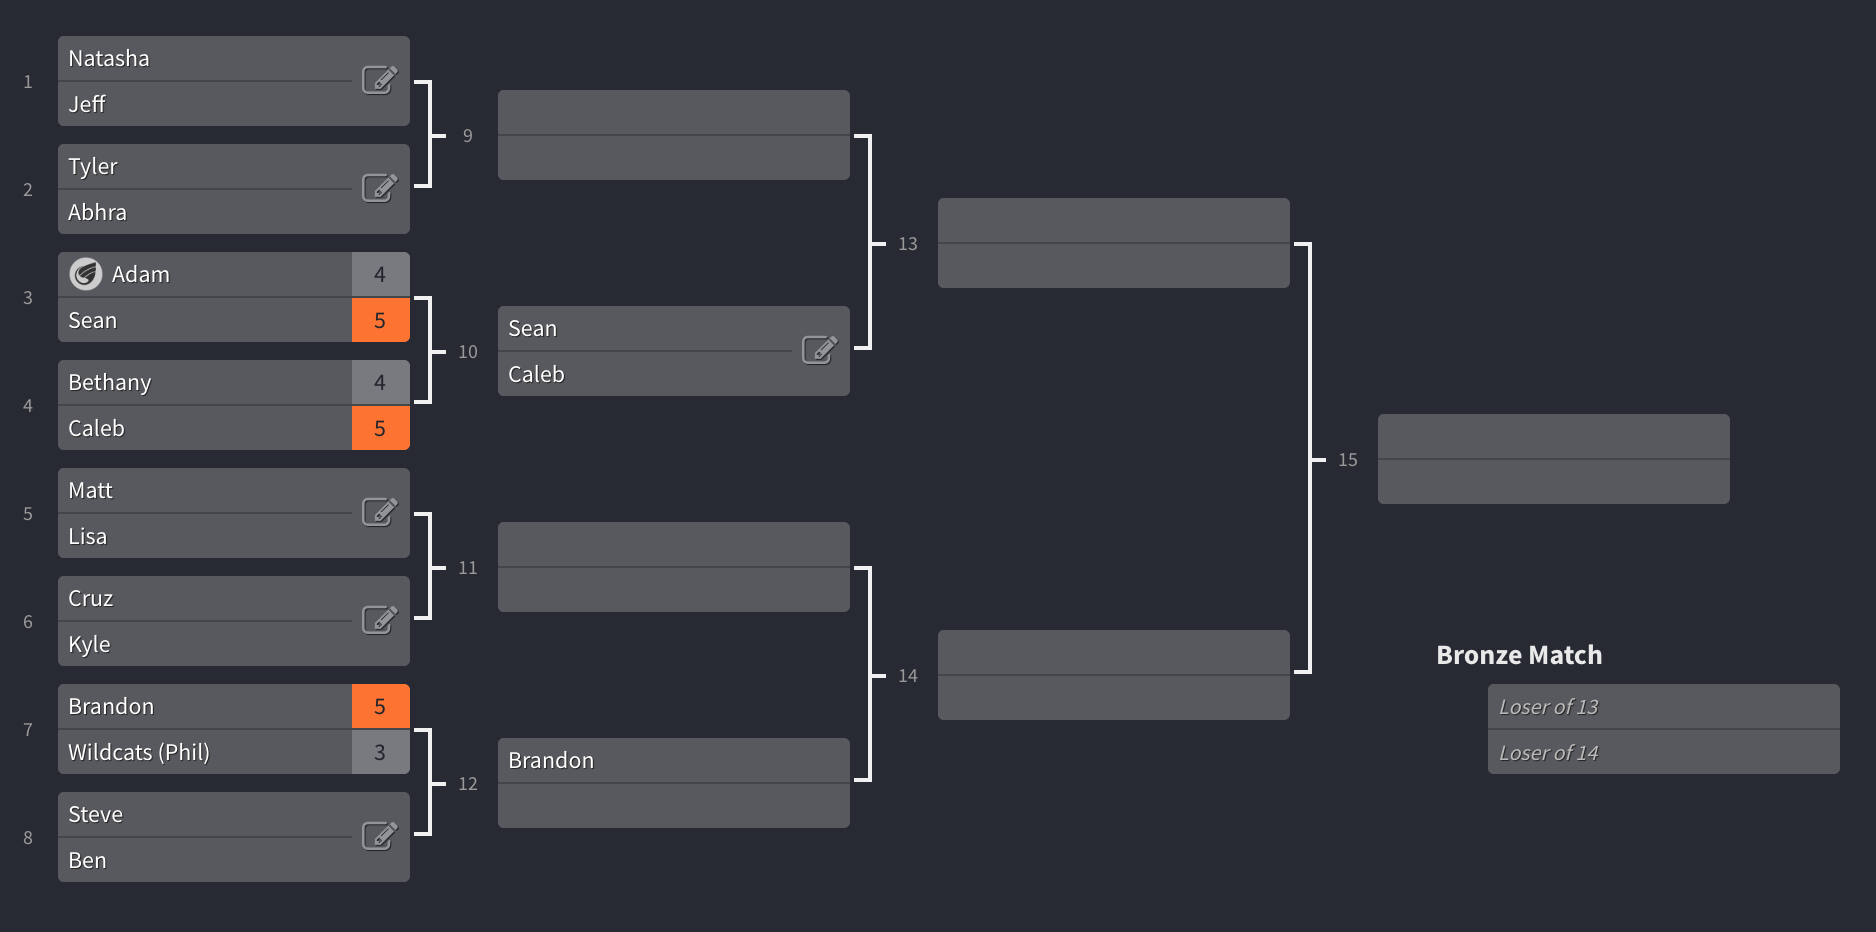
\includegraphics[width=0.9\textwidth]{fig/singles-bracket_1.png}
                \caption{Tournament bracket}
        \end{subfigure}
        \begin{subfigure}[h]{0.4\textwidth}
                \centering
                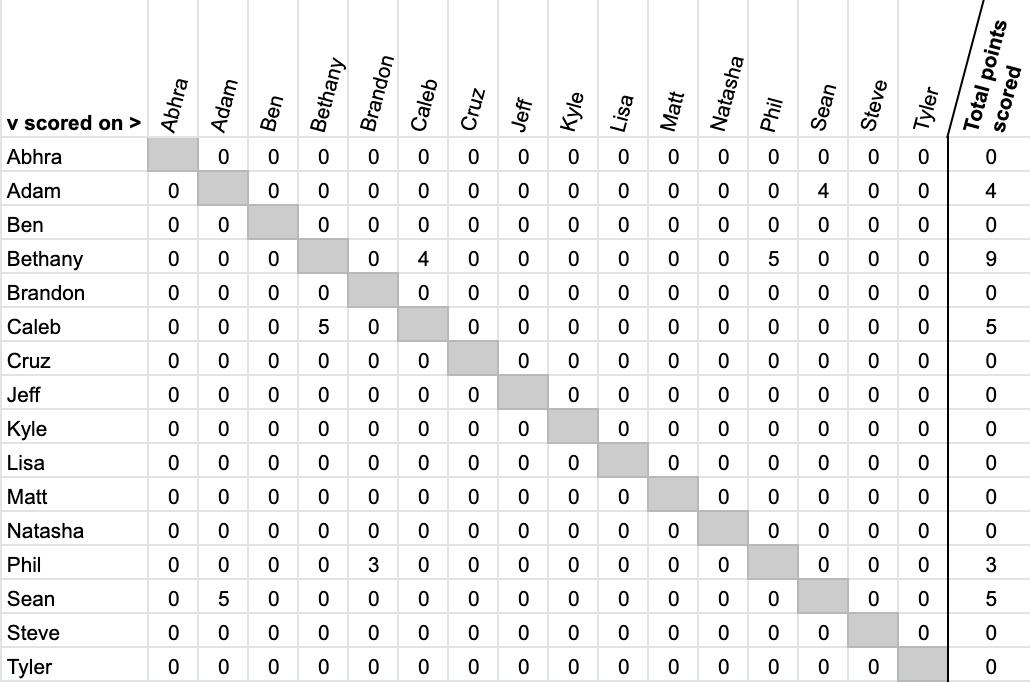
\includegraphics[width=0.9\textwidth]{fig/score-matrix_1.png}
                \caption{Score matrix}
        \end{subfigure}
        \caption{Three games are played in Round 1 of the tournament.}
\end{figure}
\begin{figure}[hb]
        \centering
        \begin{subfigure}[h]{0.5\textwidth}
        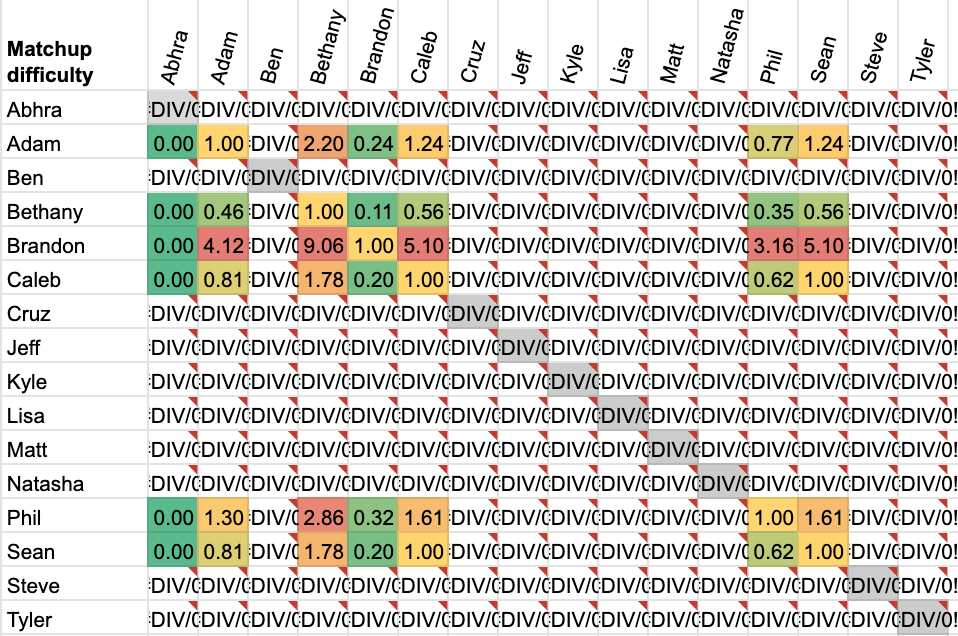
\includegraphics[width=0.9\textwidth]{fig/difficulty_1.png}
        \end{subfigure}
        \begin{subfigure}[h]{0.4\textwidth}
                \footnotesize
                \centering
                \begin{tabular}{lccc}
                        \toprule
                        Player  & $r$   & $\bar{p}$ & $k$ \\
                        \midrule
                        Abhra	& 0	& 0.00	& 0.00 \\
                        Adam	& 1	& 4.00	& 4.12 \\
                        Ben	& 0	& n/a	& n/a  \\
                        Bethany	& 1	& 4.00	& 4.12 \\
                        Brandon	& 1	& 3.00	& 3.61 \\
                        Caleb	& 1	& 5.00	& 6.40 \\
                        Cruz	& 0	& 4.25	& 5.84 \\
                        Jeff	& 0	& n/a	& n/a  \\
                        Kyle	& 0	& n/a	& n/a  \\
                        Lisa	& 0	& n/a	& n/a  \\
                        Matt	& 0	& n/a	& n/a  \\
                        Natasha	& 0	& n/a	& n/a  \\
                        Phil	& 1	& 3.00	& 3.16 \\
                        Sean	& 1	& 3.00	& 3.61 \\
                        Steve	& 0	& n/a	& n/a  \\
                        Tyler	& 0	& n/a	& n/a  \\
                        \bottomrule
                \end{tabular}
        \end{subfigure}
        \caption{Match difficulty can be predicted for matchups between 
                 any player who has completed one game.}
\end{figure}

\begin{figure}[hb]
        \centering
        \begin{subfigure}[h]{0.4\textwidth}
                \centering
                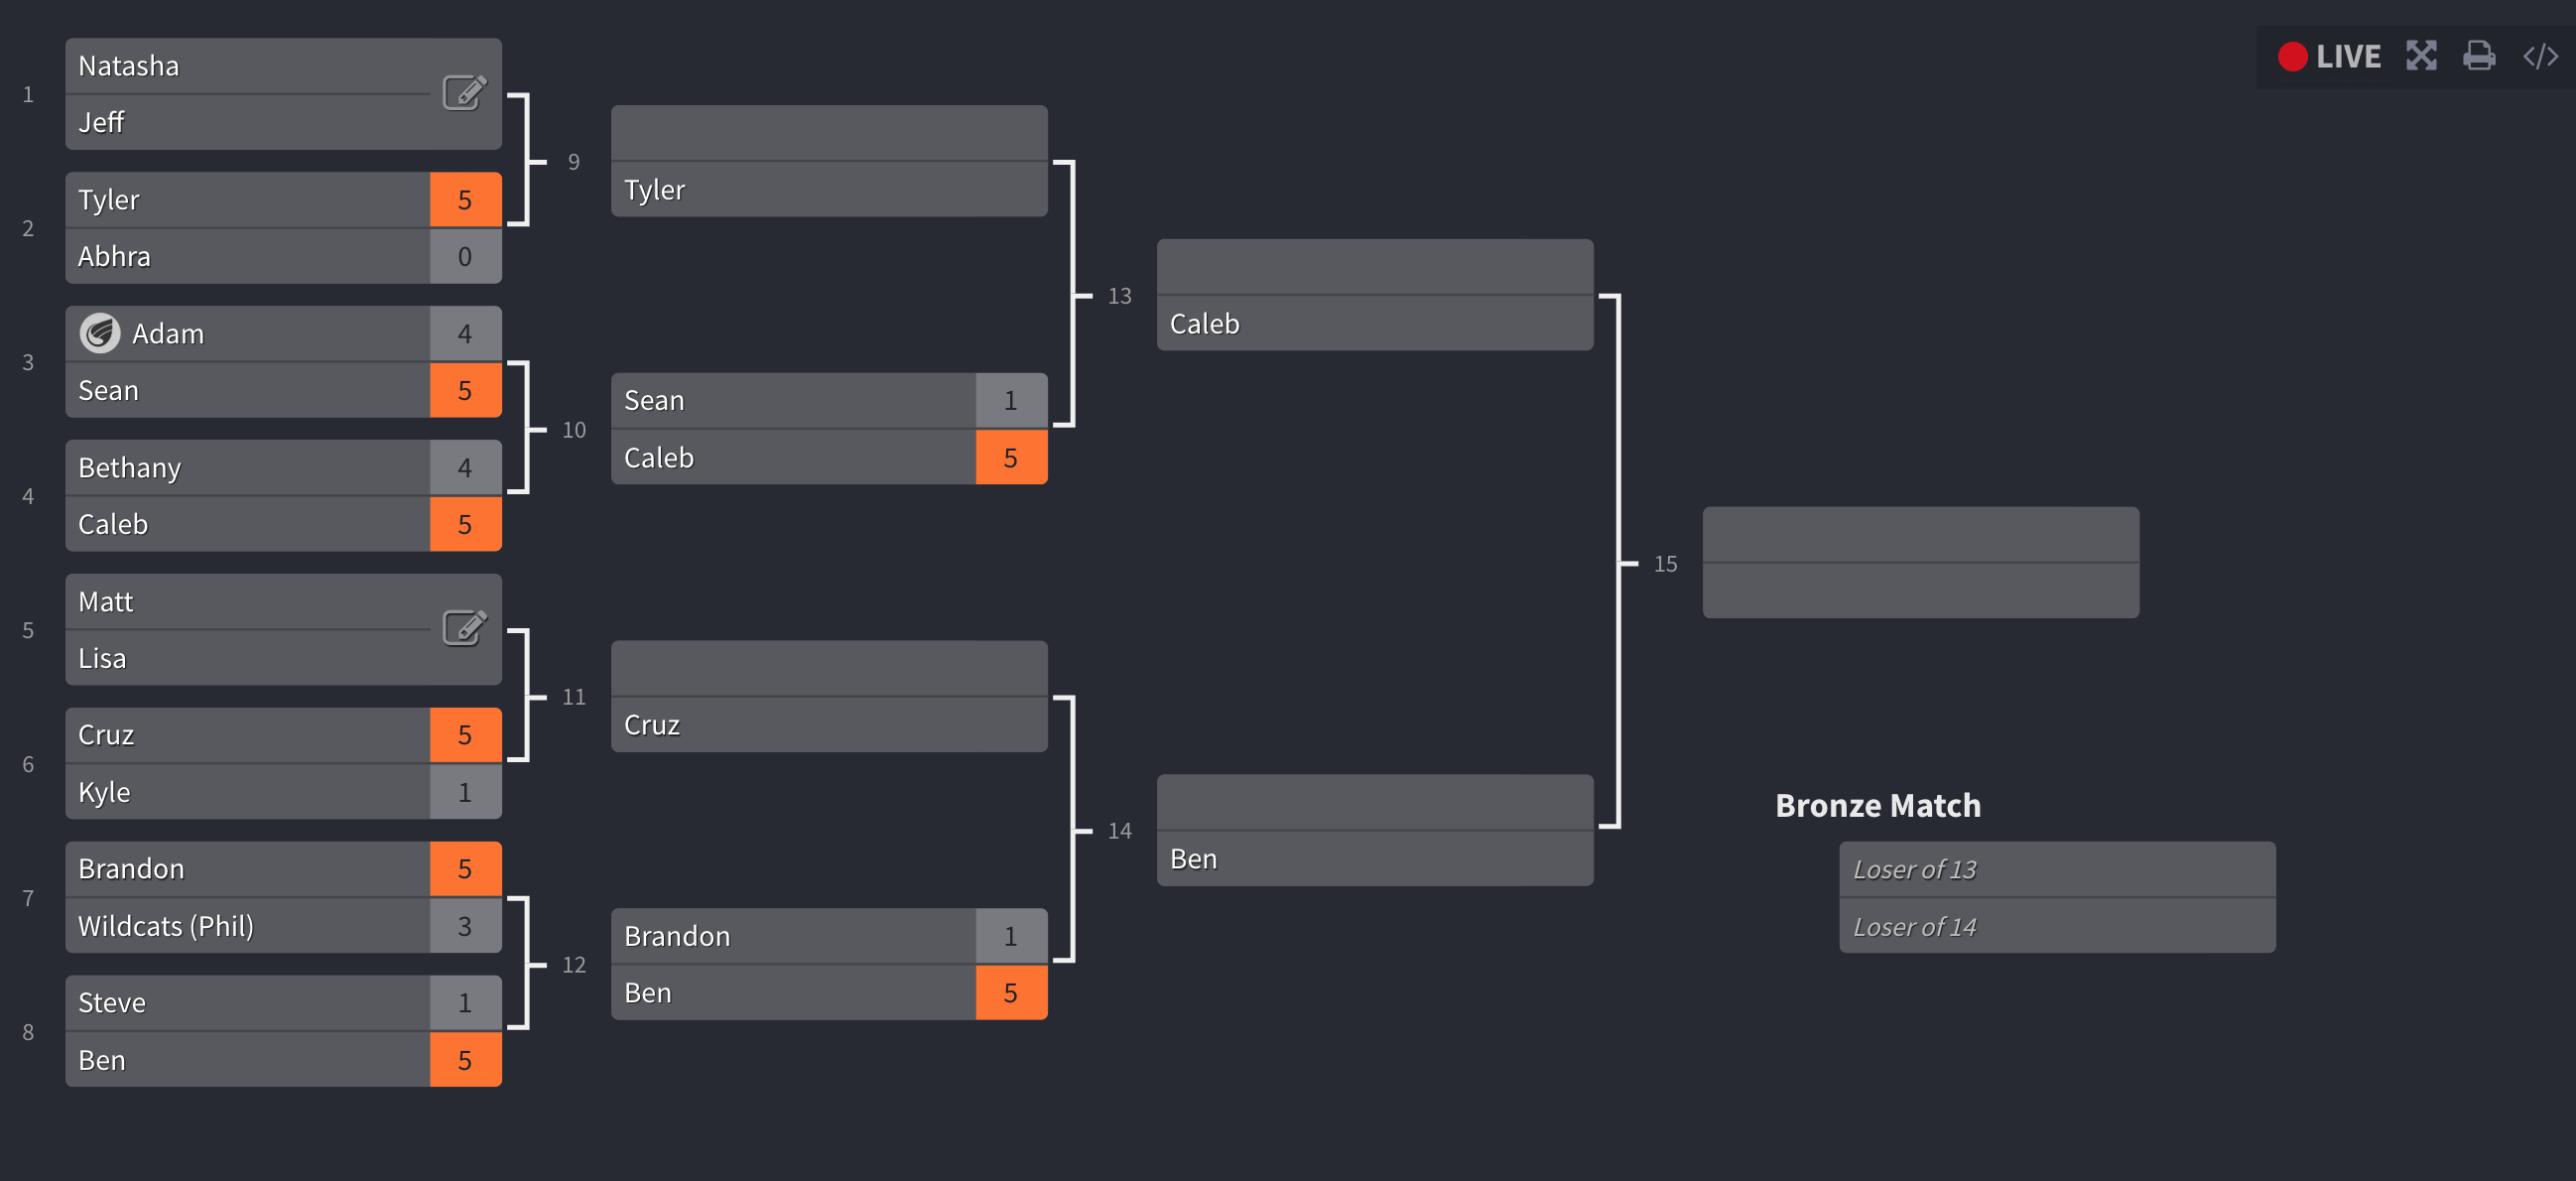
\includegraphics[width=0.9\textwidth]{fig/singles-bracket_3.png}
                \caption{Tournament bracket}
        \end{subfigure}
        \begin{subfigure}[h]{0.4\textwidth}
                \centering
                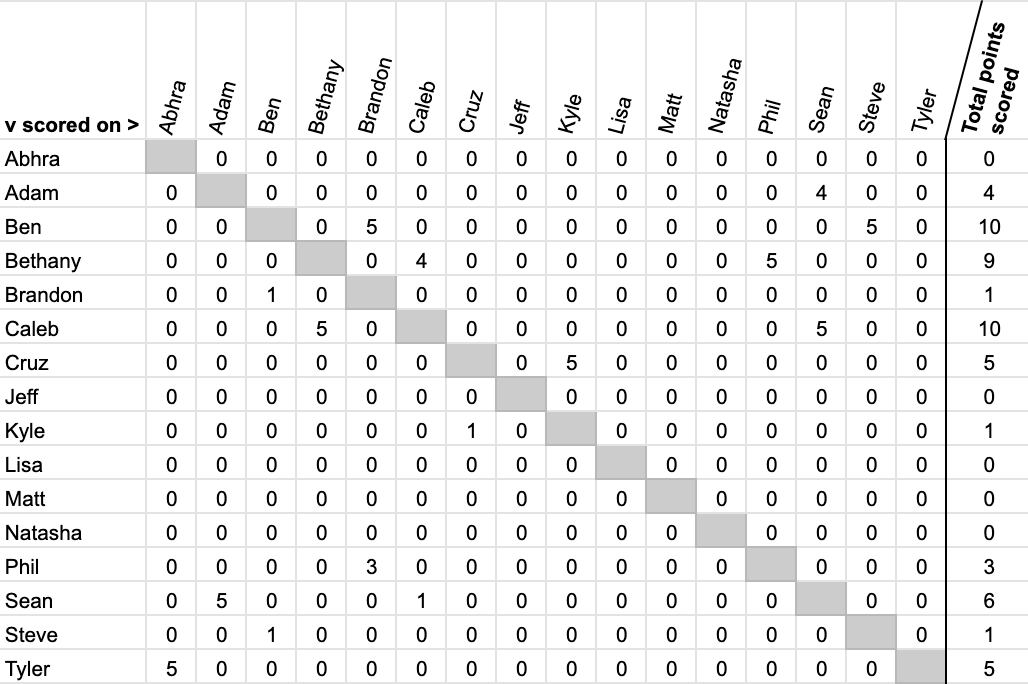
\includegraphics[width=0.9\textwidth]{fig/score-matrix_3.png}
                \caption{Score matrix}
        \end{subfigure}
        \caption{Matches in the bracket can be played asynchronously.}
\end{figure}
\begin{figure}[hb]
        \centering
        \begin{subfigure}[h]{0.5\textwidth}
                \centering
                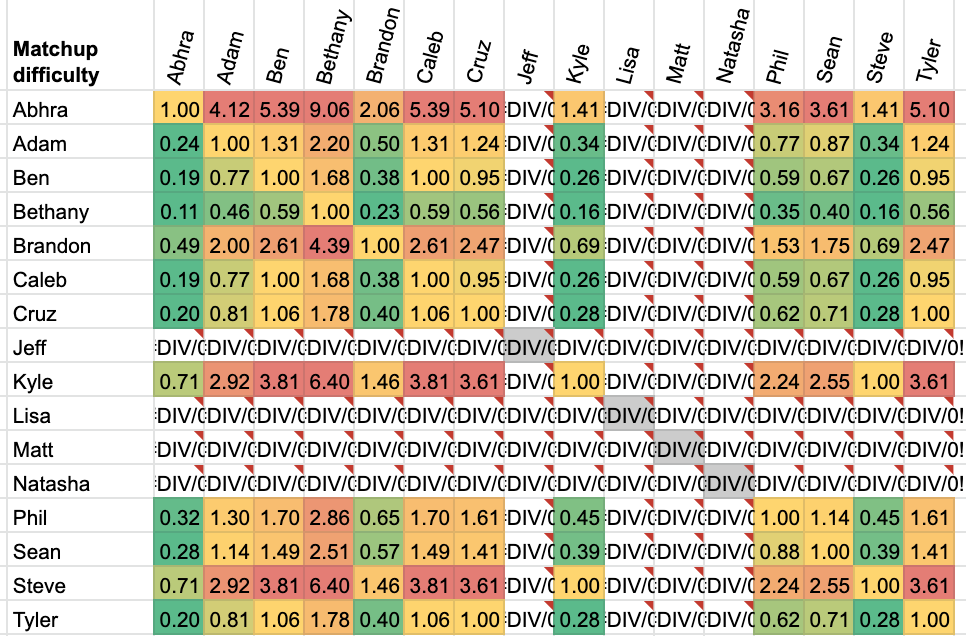
\includegraphics[width=0.9\textwidth]{fig/difficulty_3.png}
                \caption{}
        \end{subfigure}
        \begin{subfigure}[h]{0.4\textwidth}
                \footnotesize
                \centering
                \begin{tabular}{lccc}
                        \toprule
                        Player  & $r$   & $\bar{p}$ & $k$ \\
                        \midrule
                        Abhra	& 0	& 0.00	& 0.00 \\
                        Adam	& 1	& 4.00	& 4.12 \\
                        Ben	& 0	& n/a	& n/a  \\
                        Bethany	& 1	& 4.00	& 4.12 \\
                        Brandon	& 1	& 3.00	& 3.61 \\
                        Caleb	& 1	& 5.00	& 6.40 \\
                        Cruz	& 0	& 4.25	& 5.84 \\
                        Jeff	& 0	& n/a	& n/a  \\
                        Kyle	& 0	& n/a	& n/a  \\
                        Lisa	& 0	& n/a	& n/a  \\
                        Matt	& 0	& n/a	& n/a  \\
                        Natasha	& 0	& n/a	& n/a  \\
                        Phil	& 1	& 3.00	& 3.16 \\
                        Sean	& 1	& 3.00	& 3.61 \\
                        Steve	& 0	& n/a	& n/a  \\
                        Tyler	& 0	& n/a	& n/a  \\
                        \bottomrule
                \end{tabular}
        \end{subfigure}
        \caption{Since player performance is scaled by the number of matches played,
                valid predictions can be made about matchups between any player who
                has completed at least one game. HKL requires all players in the 
                tournament to play one game before can be assessed.}
\end{figure}

\subsection{Reacting to upsets}

\subsection{Predicting a winner}

\section{CASE STUDY: USING INDIVIDUAL HKL RATINGS TO CONDUCT A DOUBLES TOURNAMENT}
% Show distribution of team HKL using singles HKL for each player
% Describe how singles ratings are weighted as doubles matches are played

\subsection{Using individual ratings to form well-balanced teams}
\subsection{Using a weighted HKL to account for an individual's performance in a team environment} 

\end{document}
